%%%%%%%%%%%%%%%%%%%%%%%%%%%%%%% main.tex %%%%%%%%%%%%%%%%%%%%%%%%%%%%%%%
%                                                                      %
% ------------------ Template Relatório do IST [PT] ------------------ %
%                                                                      %
%       João Marafuz Gaspar                                            %
%       Departamento de Engenharia Eletrotécnica e de Computadores     %
%       Instituto Superior Tecnico                                     %
%       Av. Rovisco Pais                                               %
%       1049-001 Lisboa                                                %
%       Portugal                                                       %
%       E-mail: joao.marafuz.gaspar@tecnico.ulisboa.pt                 %
%                                                                      %
%  Criação:            28 de julho de 2022                             %
%  Última Modificação: 6 de abril de 2023                              %
%                                                                      %
%%%%%%%%%%%%%%%%%%%%%%%%%%%%%%%%%%%%%%%%%%%%%%%%%%%%%%%%%%%%%%%%%%%%%%%%
%  Histórico de revisões                                               %
%  v1 - 28/07/2022 - original template                                 %
%  v2 - 30/07/2022 - alteração do título do projeto para cumprir o     %
%                    projeto escrito na versão inglesa                 %
%  v3 - 06/04/2023 - alteração do tipo de letra em locais específicos, %
%                    adição de subfiguras e tabelas                    %
%%%%%%%%%%%%%%%%%%%%%%%%%%%%%%%%%%%%%%%%%%%%%%%%%%%%%%%%%%%%%%%%%%%%%%%%
%                              Preâmbulo                               %
%%%%%%%%%%%%%%%%%%%%%%%%%%%%%%%%%%%%%%%%%%%%%%%%%%%%%%%%%%%%%%%%%%%%%%%%

% ----------------------------------------------------------------------
% Configurar a classe do documento
% ----------------------------------------------------------------------
\documentclass[12pt]{article}

% ----------------------------------------------------------------------
% Definir packages externos, língua, margens, tipos de letra, novos 
% comandos e cores
% ----------------------------------------------------------------------
\usepackage[utf8]{inputenc} % Codificação utilizada
\usepackage[english]{babel} % Idioma de escrita

\usepackage[export]{adjustbox} % Alinhar imagens
\usepackage{amsmath} % Comandos extra para escrita matemática
\usepackage{amssymb} % Símbolos matemáticos
\usepackage{anysize} % Personalizar as margens
    \marginsize{2cm}{2cm}{2cm}{2cm} % {esquerda}{direita}{cima}{baixo}
\usepackage{appendix} % Apêndices
\usepackage{cancel} % Cancelar expressões
\usepackage{caption} % Legendas
    \DeclareCaptionFont{newfont}{\fontfamily{cmss}\selectfont}
    \captionsetup{labelfont={bf, newfont}}
\usepackage{cite} % Citações, tipo [1 - 3]
\usepackage{color} % Colorir texto
\usepackage{fancyhdr} % Cabeçalho e rodapé
    \pagestyle{fancy}
    \fancyhf{}
    \fancyhead[L]{\footnotesize\fontfamily{cmss}\selectfont IST} % Esquerda do cabeçalho
    \fancyhead[R]{\footnotesize\fontfamily{cmss}\selectfont ULisboa} % Direita do cabeçalho
    \fancyfoot[L]{\footnotesize\fontfamily{cmss}\selectfont Microeletronics} % Esquerda do rodapé
    \fancyfoot[C]{\thepage} % Centro do rodapé
    \fancyfoot[R]{\footnotesize\fontfamily{cmss}\selectfont LEEC} % Direita do rodapé
    \renewcommand{\footrulewidth}{0.4pt} % Régua do rodapé
\usepackage{float} % Utilizar o especificador [H] nas figuras
\usepackage{graphicx} % Imagens em LaTeX
\usepackage[colorlinks = true, plainpages = true, linkcolor = istblue, urlcolor = istblue, citecolor = istblue, anchorcolor = istblue]{hyperref}
\usepackage{indentfirst} % Primeiro parágrafo
\usepackage{siunitx} % Unidades SI
\usepackage{subcaption} % Subfiguras
\usepackage{titlesec} % Tipo de letra
    \titleformat{\section}{\fontfamily{cmss}\selectfont\Large\bfseries}{\thesection}{1em}{}
    \titleformat{\subsection}{\fontfamily{cmss}\selectfont\large\bfseries}{\thesubsection}{1em}{}
    \titleformat{\subsubsection}{\fontfamily{cmss}\selectfont\normalsize\bfseries}{\thesubsubsection}{1em}{}
    \fancyfoot[C]{\fontfamily{cmss}\selectfont\thepage}

% Encher de texto aleatório (apagar)
\usepackage{lipsum}
\usepackage{duckuments}
\usepackage[table]{xcolor}

% Novos e renovar comandos
\newcommand{\sen}{\operatorname{\sen}} % Definição da função seno
\newcommand{\HRule}{\rule{\linewidth}{0.5mm}} % Definição de uma régua
\renewcommand{\appendixpagename}{\LARGE \fontfamily{cmss}\selectfont Apêndices}
\renewcommand{\appendixtocname}{Apêndices}

% Cores
\definecolor{istblue}{RGB}{3, 171, 230}
\definecolor{dkgreen}{rgb}{0,0.6,0}
\definecolor{gray}{rgb}{0.5,0.5,0.5}

%%%%%%%%%%%%%%%%%%%%%%%%%%%%%%%%%%%%%%%%%%%%%%%%%%%%%%%%%%%%%%%%%%%%%%%%
%                               Documento                              %
%%%%%%%%%%%%%%%%%%%%%%%%%%%%%%%%%%%%%%%%%%%%%%%%%%%%%%%%%%%%%%%%%%%%%%%%
\begin{document}

% ----------------------------------------------------------------------
% Capa
% ----------------------------------------------------------------------
\begin{center}
    \begin{figure}
        \vspace{-1.0cm}
        
\includegraphics[scale = 0.3, left]{Imagens/IST_A.eps} % Tipo de assinatura do IST
    \end{figure}
    \mbox{}\\[2.0cm]
    \textsc{\Huge Projeto de Sistemas Digitais}\\[2.5cm]
    \textsc{\LARGE LEEC}\\[2.0cm]
    \HRule\\[0.4cm]
    {\large \bf {\fontfamily{cmss}\selectfont } [\texttt{EN}]}\\[0.2cm]
    \HRule\\[1.5cm]
\end{center}

\begin{flushleft}
    \textbf{\fontfamily{cmss}\selectfont Authors:}
\end{flushleft}

\begin{center}
    \begin{minipage}{0.4\textwidth}
        \begin{flushleft}
            Alexandre Santos (99884)\\
            Nuno Abreu (103416)\\
            Carlos Reis()\\
        \end{flushleft}
    \end{minipage}%
    \begin{minipage}{0.6\textwidth}
        \begin{flushright}
            \href{mailto:ares.santos@tecnico.ulisboa.pt}{\texttt{ares.santos@tecnico.ulisboa.pt}}\\
            \href{mailto:nuno.g.tribolet.de.abreu@tecnico.ulisboa.pt}{\texttt{nuno.g.tribolet.de.abreu@tecnico.ulisboa.pt}}\\
            \href{mailto:guilherme.garcia@tecnico.ulisboa.pt}{\texttt{guilherme.garcia@tecnico.ulisboa.pt}}\\
            
        \end{flushright}
    \end{minipage}


\end{center}
    
\begin{flushleft}
    \large $\boxed{\text{\bf \fontfamily{cmss}\selectfont Group 10}}$\\[4.0cm]
\end{flushleft}
    
\begin{center}
    \large \bf \fontfamily{cmss}\selectfont 2023/2024 -- 2nd Semester, P4
\end{center}

\thispagestyle{empty}

\setcounter{page}{0}

\newpage

% ----------------------------------------------------------------------
% Conteúdo
% ----------------------------------------------------------------------
\tableofcontents 

\newpage
%%%%%%%%%%%%%%    Abstract           %%%%%%%%%%%%%%%%%

\section{Abstract}
The following report pertains to the first laboratory task of Project of Digital Systems.

The objective is to design and implement a simple logic-arithmetic calculator, utilizing VHDL hardware description language and making use of simulation and logic synthesis. 
To achieve this objective a data-path , control unit and an interface
unit to integrate the design with the FPGA(Basys3 Digilent development board) where created. 

The calculator performs addition , subtraction , multiplication, AND (for logic operation), rotate-left  (for shift operation), load operation in register 1 and register 2. All the operations are done utilising an arithmetic-logic unit (ALU) , multipliers (MUL), two registers(REG's) and two multiplexers(MUX's). The calculator works with number's between -512 to 511. 

The design was then tested on the FPGA to ensure that the calculator performs all the operations that it was designed for.

%%%%%%%%%%%%%%%%%%%%  Datapath   %%%%%%%%%%%%%%%%%%%%%%%%%%%%%%%%%%%%%%%%%%%%%%%
\section{Datapath}

The datapath component is the main processing unit of the circuit. It follows the schematic present in the lab assignment document, which has been modified in \ref{fig:datapath} to also show the input control signals of the component.

\begin{figure}[H]
	\centering
	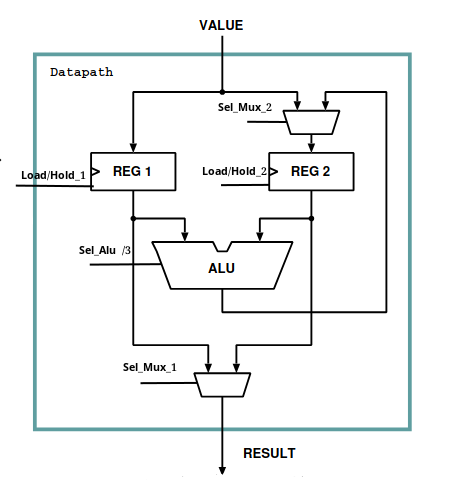
\includegraphics[width=0.6\linewidth]{Imagens/datapath.png}
	\caption{Schematic of the datapath component}
	\label{fig:datapath}
\end{figure}

The ALU block in the schematic has been implemented as follows:

\begin{figure}[H]
	\centering
	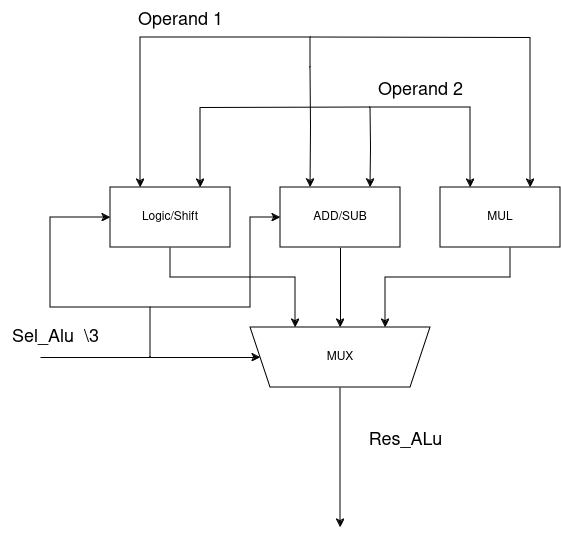
\includegraphics[width=0.8\linewidth]{Imagens/ALU.png}
	\caption{Schematic of the ALU block}
	\label{fig:ALU}
\end{figure}

Both registers are positive edge triggered and are controlled by a Load/Hold bit. Their output is represented in table \ref{tab:Reg}. Register 1 is a 10 bit register and register 2 is a 16 bit register. Apart from that their behaviour is the same.

\begin{table}[H]
	\center
	\begin{tabular}{|c|c|c|c|}
		\hline
		Reset & Load/Hold & Clk        & Behaviour \\
		\hline
		1     & X         & $\uparrow$ & Reset     \\
		0     & 1         & $\uparrow$ & Load      \\
		0     & 0         & $\uparrow$ & Hold      \\
		\hline
	\end{tabular}
	\caption{register behaviour table}
	\label{tab:Reg}
\end{table}

The ALU's behaviour depends on the control signal "Sel\_Alu" which is a three wide control vector. The ALU expects a 10 bit and 16 bit operand as operand 1 and operand 2 respectively. Its behavious is described in table \ref{tab:ALU}. Since we are group 10, in accordance with the lab assignment our shift operation is a rotate-left and our logic operation is an AND.

\begin{table}[H]
	\center
	\begin{tabular}{|c|c|c|}
		\hline
		Sel\_ALU & Clk        & Behaviour       \\
		\hline
		1XX     & $\uparrow$ & $A \times B$ \\
		000     & $\uparrow$ & $A-B$        \\
		001     & $\uparrow$ & $A+B$        \\
		010     & $\uparrow$ & Shift        \\
		011     & $\uparrow$ & Logic        \\
		\hline
	\end{tabular}
	\caption{ALU behaviour table. A and B refer to operand 1 and 2.}
	\label{tab:ALU}
\end{table}

The multiplexers are both 16 bit. Since the circuit's input is 10 bits wide, signal aware padding was done on multiplexer 2's connection with the circuits input, i.e. the 6 higher order bits were made the same as the signal bit.
The multiplexers are controlled by their respective "Sel\_Mul" control signals.

%%%%%%%%%%%%%%%%%%%      Control Unit       %%%%%%%%%%%%%%%%%%%%%%%%%%%%%%%%%%%%
\newpage
\section{Control Unit}
%Parte do Carlos
For the control unit of the circuit we designed a Moore Finite State Machine.
the inputs of the circuit are push-buttons that command different operations. Therefore, quick changes in inputs(release of the buttons) are to be expected with little to no influence on the control's output. Hence, the choice of Moore machine with each state corresponding to :

-waiting for instruction, 

-performing instruction,

-preparing for next instruction.

The state diagram implemented is below[\ref{fig:FSM}]:
\begin{figure}[H]
	\centering
	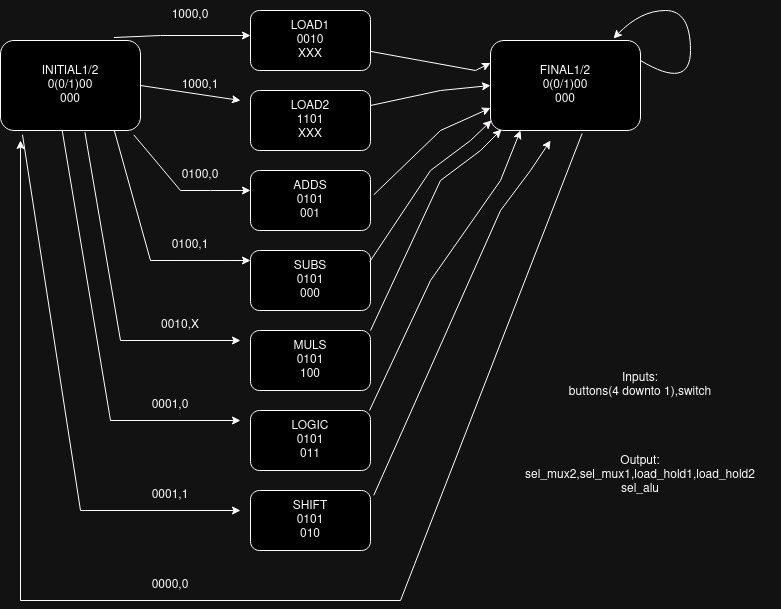
\includegraphics[width=0.8\linewidth]{Imagens/state_machine_lab1.jpg}
	\caption{State machine for control unit}
	\label{fig:FSM}
\end{figure}

There is one different state for each instruction. Each instruction takes up one clock cycle so the control unit needs only maintain these operation states for only one clock cycle, after which it transitions to a final state where it waits for no input,the FINAL(avoiding more than one button or operation command at once). After all inputs have been removed(no buttons pressed) the machine transitions to INITAL where it awaits for the next instruction.Only when at the INITAL state does the machine accept commands from the user(buttons pressed).

Both INITIAL and FINAL have two variations, INITIAL1/INITIAL2 and FINAL1/FINAL2. These variations allow for different registered values to be presented at the display. A LOAD1 should present the value of register\_1 at the display and LOAD2 should present the value at register\_2.

The circuit implemented has one VHDL process corresponding to one register that stores the current state(curr\_state). The next state is calculated with a combinatorial logic circuit(concurrent VHDL commands). This allows the calculation of next state and transitioning at each clock cycle, a necessary feature since we expect the operation states to last only that time.

Our first implementation with three VHDL processes produced two registers(curr\_state, next\_state) which made each state last for two clock cycles. Although some operations such as LOAD1 and LOAD2 were unaffected, these architecture failed to execute any arithmetic and logic operations since the command signals would last for twice as long as intended resulting in repeated operations.

The commanding signals(outputs of the control unit) are 4 bits for multiplexer selection and register enabling(sel\_mux2, sel\_mux1 , load\_hold1, load\_hold2) and three bits for selecting one of 5 operations at the ALU.

sel\_mux1 is responsible for the display- '0' wil show the value at register1 and '1' wil show the value at register2.
sel\_mux2 is responsible for the input of register2 - '0' will connect it to the ALU output and '1' will connect it to the data input. Only at LOAD2 will this take the value '1'. load\_hold1 is the enable for the register\_1, only at LOAD1 will it be '1'. load\_hold2 is the enable for register2. register2 is updated(enabled) at all states except INITIAL, FINAL and LOAD1.


\begin{table}[H]
	\centering
	\begin{tabular}{cccccc}
		STATE & sel\_mux2 & sel\_mux1 & load\_hold1 & load\_hold2 & sel\_alu\\
		ADDS    & 0 & 1 & 0 & 1 & 001\\
		SUBS    & 0 & 1 & 0 & 1 & 000\\
		MULS    & 0 & 1 & 0 & 1 & 100\\
		LOGIC   & 0 & 1 & 0 & 1 & 011\\
		SHIFT   & 0 & 1 & 0 & 1 & 010\\
		LOAD1   & 0 & 0 & 1 & 0 & XXX\\
		LOAD2   & 1 & 1 & 0 & 1 & XXX\\
		INITIAL & 0 & 0/1 & 0 & 0 & 000\\
		FINAL   & 0 & 0/1 & 0 & 0 & 000\\
	\end{tabular}
	\caption{Control signals per operation}
	\label{tab:my_label}
\end{table}

The 5 ALU operations were selected with the signals 000, 001, 010, 011 and 100. At first, the command MULS(100) was associated with 1XX(dont care values) but this turned out to be bad design since the datapath unit was unable to recognise signals with X. Although the control unit can use these bits for optimization of the truth tables it implements, special attention is required at the datapath inputs to avoid having unspecified situations(all possible inputs must have a specified response). For simplicity, the value of 100 at the ALU selection was associated to the MULS operation.

%%%%%%%%%%%%%%%%%%%      Overall Circuit  Performance        %%%%%%%%%%%%%%%%%%%
%Parte do Nuno
\section{Test-bench and Simulation}
With the calculator data-path and control unit implemented, a test-bench was made to simulate and analyse the calculator performance. 

Following the project assignment the buttons were associated to the operations as  can be seen in table \ref{BUTTONS}:

\begin{table}[H]
	\centering
	\begin{tabular}{|c|c|c|}
        \hline
		    & Switch = 0 & Switch = 1\\
      \hline
		  BTNL  & LOAD REG1 & LOAD REG2 \\
    \hline
		BTNU    & ADD & SUB\\
    \hline
		BTNR    & MUL & MUL \\
    \hline
		BTND   & AND & ROTATE LEFT\\
    \hline
        BTNC   & RESET & RESET \\
        \hline
		
	\end{tabular}
	\caption{Buttons assignments}
	\label{BUTTONS}
\end{table}

To simplify the results of the behavioral simulation the table \ref{tab:simulation} was made. The clock cycle as a period of 10 ns and every instance that something is change it will appear in the simulation table. The value showned for Reg1 , Reg2, Display and $Data\textunderscore in$ are in hexadecimal format.

In the beginning of the simulation $Data\textunderscore in$, Reg1, Reg2 and Display are undefined with the symbols "UUU". Reg 1 ,Reg2 and Display are then set to zero as the reset is pressed setting Reg1 and Reg2 to zero, therefore Display is also set to zero. $Data\textunderscore in$ is only defined when some value is inputted. 

To test the loads 8 is loaded in Reg1 by pressing BTNL, this process also displays 8 in the Display. Then switch is activated to load 6 in Reg2 by pressing BTNL, also then displaying 6 in the Display.

With the initial numbers loaded we then test all the operation. Starting by subtracting 6 to 8 and placing the result (2) in Reg2. We then add 8 with 2 and store the result, A(10 in decimal), in Reg2. The next operation done is multiplication between 8 and a , resulting with the value 50 (80 in decimal) stored in Reg2. The operation And , our logic operation, is then done between 8 and 50 saving the output signal in Reg2. For the final operation we did a rotate left,our shift operation, to the number stored in Reg1(8 in decimal / 100 in binary) and saved the output in Reg2 with the value 10(16 in decimal / 1000 in binary). 

All the operations were done with success and the calculator behaved as designed. Therefore we advanced to the Post-Synthesis Timing Simulation that had the same output and behaviour as the Behavioral Simulation. 

Achieving the expected outcome of both simulations we then advanced to the test in the FPGA board.

\begin{table}[H]
   
    \hskip-1.0cm\begin{tabular}{|l|l|l|l|l|l|l|l|l|l|l|l|}
    \hline
        t(ns) & State & $Data\textunderscore in$  & Reg1 & Reg2 & Switch & BTNL & BTNU & BTNR & BTND& BTNC& Display\\
        \hline
        200 & Initial1 & UUU & UUU&UUU&0&0&0&0&0&0&UUU\\
        \hline
         220 & Initial1 & UUU & UUU&UUU&0&0&0&0&0&1&UUU\\
        \hline
         225 & Final2 & UUU & UUU&UUU&0&0&0&0&0&1&UUU\\
        \hline
        240 & Final2 & UUU & UUU&UUU&0&0&0&0&0&0&UUU\\
        \hline
        245 & Initial2 & UUU & 0&0&0&0&0&0&0&0&0\\
        \hline
        280 & Initial2 & 8 & 0&0&0&1&0&0&0&0&0\\
        \hline
        285 & LOAD1 & 8 & 0&0&0&1&0&0&0&0&0\\
        \hline
        295 & Final1 & 8 & 8&0&0&1&0&0&0&0&8\\
        \hline
        300 & Final1 & 8 & 8&0&0&0&0&0&0&0&8\\
        \hline
        305 & Initial1 & 8 & 8&0&0&0&0&0&0&0&8\\
        \hline
        320 & Initial1 & 8 & 8&0&1&0&0&0&0&0&8\\
        \hline
        340 & Initial1 & 6 & 8&0&1&0&0&0&0&0&8\\
        \hline
        360 & Initial1 & 6 & 8&0&1&1&0&0&0&0&8\\
        \hline
        365 & LOAD2 & 6 & 8&0&1&1&0&0&0&0&0\\
        \hline
        375 & Final2 & 6 & 8&6&1&1&0&0&0&0&6\\
        \hline
        380 & Final2 & 6 & 8&6&1&0&0&0&0&0&6\\
        \hline
        385 & Initial2 & 6 & 8&6&1&0&0&0&0&0&6\\
        \hline
        440 & Initial2 & 6 & 8&6&1&0&1&0&0&0&6\\
        \hline
        445 & Subs & 6 & 8&6&1&0&1&0&0&0&6\\
        \hline
        455 & Final2 & 6 & 8&2&1&0&1&0&0&0&2\\
        \hline
        460 & Final2 & 6 & 8&2&0&0&0&0&0&0&2\\
        \hline
        465 & Initial2 & 6 & 8&2&0&0&0&0&0&0&2\\
        \hline
        520 & Initial2 & 6 & 8&2&0&0&1&0&0&0&2\\
        \hline
        525 & Adds& 6 & 8&2&0&0&1&0&0&0&2\\
        \hline
        535 & Final2& 6 & 8&A&0&0&1&0&0&0&A\\
        \hline
        540 & Final2& 6 & 8&A&0&0&0&0&0&0&A\\
        \hline
        545 & Initial2& 6 & 8&A&0&0&0&0&0&0&A\\
        \hline
        600 & Initial2& 6 & 8&A&0&0&0&1&0&0&A\\
        \hline
        605 & Muls& 6 & 8&A&0&0&0&1&0&0&A\\
        \hline
        615 & Final2& 6 & 8&50&0&0&0&1&0&0&50\\
        \hline
        620 & Final2& 6 & 8&50&0&0&0&0&0&0&50\\
        \hline
        625 & Initial2& 6 & 8&50&0&0&0&0&0&0&50\\
        \hline
        680 & Initial2& 6 & 8&50&0&0&0&0&1&0&50\\
        \hline
        685 & Logic& 6 & 8&50&0&0&0&0&1&0&50\\
        \hline
        695 & Final2& 6 & 8&0&0&0&0&0&1&0&0\\
        \hline
        700 & Final2& 6 & 8&0&0&0&0&0&0&0&0\\
        \hline
        705 & Initial2& 6 & 8&0&0&0&0&0&0&0&0\\
        \hline
        720 & Initial2& 6 & 8&0&1&0&0&0&0&0&0\\
        \hline
        760 & Initial2& 6 & 8&0&1&0&0&0&1&0&0\\
        \hline
        765 & Shift& 6 & 8&0&1&0&0&0&1&0&0\\
        \hline
        775 & Final2& 6 & 8&10&1&0&0&0&1&0&10\\
        \hline
        780 & Final2& 6 & 8&10&1&0&0&0&0&0&10\\
        \hline
        785 & Initial2& 6 & 8&10&1&0&0&0&0&0&10\\
        \hline
        
    \end{tabular}
    \caption{Simulation Table}
    \label{tab:simulation}
     
\end{table}



\section{Physical implementation results}

%%%%%%%%%%%%%%%%%%%      Conclusion                  %%%%%%%%%%%%%%%%%%%%%%%%%%%
%Mais parte do Nuno
\section{Conclusion}

Through this laboratory we successfully integrated a datapath and control unit components to achieve a functioning basic calculator that was according to specifications.

We integrated both components using a hierarchical structure and a "circuit" component that correctly connects the datapath and control unit.

We simulated the final circuit to test if its behaviour was as designed. This allowed us to find errors in our design and correct them in timely manner.


\end{document}

